\documentclass[twoside]{book}

% Packages required by doxygen
\usepackage{fixltx2e}
\usepackage{calc}
\usepackage{doxygen}
\usepackage[export]{adjustbox} % also loads graphicx
\usepackage{graphicx}
\usepackage[utf8]{inputenc}
\usepackage{makeidx}
\usepackage{multicol}
\usepackage{multirow}
\PassOptionsToPackage{warn}{textcomp}
\usepackage{textcomp}
\usepackage[nointegrals]{wasysym}
\usepackage[table]{xcolor}

% Font selection
\usepackage[T1]{fontenc}
\usepackage[scaled=.90]{helvet}
\usepackage{courier}
\usepackage{amssymb}
\usepackage{sectsty}
\renewcommand{\familydefault}{\sfdefault}
\allsectionsfont{%
  \fontseries{bc}\selectfont%
  \color{darkgray}%
}
\renewcommand{\DoxyLabelFont}{%
  \fontseries{bc}\selectfont%
  \color{darkgray}%
}
\newcommand{\+}{\discretionary{\mbox{\scriptsize$\hookleftarrow$}}{}{}}

% Page & text layout
\usepackage{geometry}
\geometry{%
  a4paper,%
  top=2.5cm,%
  bottom=2.5cm,%
  left=2.5cm,%
  right=2.5cm%
}
\tolerance=750
\hfuzz=15pt
\hbadness=750
\setlength{\emergencystretch}{15pt}
\setlength{\parindent}{0cm}
\setlength{\parskip}{3ex plus 2ex minus 2ex}
\makeatletter
\renewcommand{\paragraph}{%
  \@startsection{paragraph}{4}{0ex}{-1.0ex}{1.0ex}{%
    \normalfont\normalsize\bfseries\SS@parafont%
  }%
}
\renewcommand{\subparagraph}{%
  \@startsection{subparagraph}{5}{0ex}{-1.0ex}{1.0ex}{%
    \normalfont\normalsize\bfseries\SS@subparafont%
  }%
}
\makeatother

% Headers & footers
\usepackage{fancyhdr}
\pagestyle{fancyplain}
\fancyhead[LE]{\fancyplain{}{\bfseries\thepage}}
\fancyhead[CE]{\fancyplain{}{}}
\fancyhead[RE]{\fancyplain{}{\bfseries\leftmark}}
\fancyhead[LO]{\fancyplain{}{\bfseries\rightmark}}
\fancyhead[CO]{\fancyplain{}{}}
\fancyhead[RO]{\fancyplain{}{\bfseries\thepage}}
\fancyfoot[LE]{\fancyplain{}{}}
\fancyfoot[CE]{\fancyplain{}{}}
\fancyfoot[RE]{\fancyplain{}{\bfseries\scriptsize Generated by Doxygen }}
\fancyfoot[LO]{\fancyplain{}{\bfseries\scriptsize Generated by Doxygen }}
\fancyfoot[CO]{\fancyplain{}{}}
\fancyfoot[RO]{\fancyplain{}{}}
\renewcommand{\footrulewidth}{0.4pt}
\renewcommand{\chaptermark}[1]{%
  \markboth{#1}{}%
}
\renewcommand{\sectionmark}[1]{%
  \markright{\thesection\ #1}%
}

% Indices & bibliography
\usepackage{natbib}
\usepackage[titles]{tocloft}
\setcounter{tocdepth}{3}
\setcounter{secnumdepth}{5}
\makeindex

% Hyperlinks (required, but should be loaded last)
\usepackage{ifpdf}
\ifpdf
  \usepackage[pdftex,pagebackref=true]{hyperref}
\else
  \usepackage[ps2pdf,pagebackref=true]{hyperref}
\fi
\hypersetup{%
  colorlinks=true,%
  linkcolor=blue,%
  citecolor=blue,%
  unicode%
}

% Custom commands
\newcommand{\clearemptydoublepage}{%
  \newpage{\pagestyle{empty}\cleardoublepage}%
}

\usepackage{caption}
\captionsetup{labelsep=space,justification=centering,font={bf},singlelinecheck=off,skip=4pt,position=top}

%===== C O N T E N T S =====

\begin{document}

% Titlepage & ToC
\hypersetup{pageanchor=false,
             bookmarksnumbered=true,
             pdfencoding=unicode
            }
\pagenumbering{alph}
\begin{titlepage}
\vspace*{7cm}
\begin{center}%
{\Large Line Segment Intersector \\[1ex]\large 1.\+0 }\\
\vspace*{1cm}
{\large Generated by Doxygen 1.8.13}\\
\end{center}
\end{titlepage}
\clearemptydoublepage
\pagenumbering{roman}
\tableofcontents
\clearemptydoublepage
\pagenumbering{arabic}
\hypersetup{pageanchor=true}

%--- Begin generated contents ---
\chapter{Hierarchical Index}
\section{Class Hierarchy}
This inheritance list is sorted roughly, but not completely, alphabetically\+:\begin{DoxyCompactList}
\item \contentsline{section}{Event\+Queue$<$ T $>$}{\pageref{classEventQueue}}{}
\item \contentsline{section}{Event\+Queue$<$ Line\+Segment\+Intersector\+:\+:L\+S\+I\+Point $>$}{\pageref{classEventQueue}}{}
\item \contentsline{section}{Graphix}{\pageref{classGraphix}}{}
\begin{DoxyCompactList}
\item \contentsline{section}{L\+S\+I\+Graphix}{\pageref{classLSIGraphix}}{}
\end{DoxyCompactList}
\item \contentsline{section}{Line\+Segment}{\pageref{classLineSegment}}{}
\item \contentsline{section}{Line\+Segment\+Intersector}{\pageref{classLineSegmentIntersector}}{}
\item \contentsline{section}{Point}{\pageref{classPoint}}{}
\item \contentsline{section}{Status$<$ T $>$}{\pageref{classStatus}}{}
\item \contentsline{section}{Status$<$ L\+S\+I\+Segment $>$}{\pageref{classStatus}}{}
\end{DoxyCompactList}

\chapter{Class Index}
\section{Class List}
Here are the classes, structs, unions and interfaces with brief descriptions\+:\begin{DoxyCompactList}
\item\contentsline{section}{\hyperlink{classEventQueue}{Event\+Queue$<$ T $>$} }{\pageref{classEventQueue}}{}
\item\contentsline{section}{\hyperlink{classGraphix}{Graphix} \\*Class for handling graphics using Open\+GL }{\pageref{classGraphix}}{}
\item\contentsline{section}{\hyperlink{classLineSegment}{Line\+Segment} \\*Class for line segments }{\pageref{classLineSegment}}{}
\item\contentsline{section}{\hyperlink{classLineSegmentIntersector}{Line\+Segment\+Intersector} }{\pageref{classLineSegmentIntersector}}{}
\item\contentsline{section}{\hyperlink{classLSIGraphix}{L\+S\+I\+Graphix} \\*Class for especially handling events for Bentley-\/\+Ottoman Algorithm. Inherits \hyperlink{classGraphix}{Graphix} class }{\pageref{classLSIGraphix}}{}
\item\contentsline{section}{\hyperlink{classPoint}{Point} \\*Stores point with X \& Y coordinate }{\pageref{classPoint}}{}
\item\contentsline{section}{\hyperlink{classStatus}{Status$<$ T $>$} }{\pageref{classStatus}}{}
\end{DoxyCompactList}

\chapter{Class Documentation}
\hypertarget{classEventQueue}{}\section{Event\+Queue$<$ T $>$ Class Template Reference}
\label{classEventQueue}\index{Event\+Queue$<$ T $>$@{Event\+Queue$<$ T $>$}}


{\ttfamily \#include $<$Event\+Queue.\+h$>$}

\subsection*{Public Member Functions}
\begin{DoxyCompactItemize}
\item 
T \hyperlink{classEventQueue_aa2f631077b7f200f65fb87bd3bb60f71}{extract\+Min} ()
\item 
T \hyperlink{classEventQueue_a3e739a353e6ef3fac228a33dd483d730}{peek} ()
\item 
void \hyperlink{classEventQueue_a516dc912aae6d1505ed912fc50f7c33a}{insert} (T k)
\item 
int \hyperlink{classEventQueue_a0ce7b577678a2d182edcf24fdc91397e}{size} ()
\end{DoxyCompactItemize}


\subsection{Detailed Description}
\subsubsection*{template$<$class T$>$\newline
class Event\+Queue$<$ T $>$}

The event queue is a min heap 
\begin{DoxyTemplParams}{Template Parameters}
{\em T} & class needs $<$ function and defined \\
\hline
\end{DoxyTemplParams}


\subsection{Member Function Documentation}
\mbox{\Hypertarget{classEventQueue_aa2f631077b7f200f65fb87bd3bb60f71}\label{classEventQueue_aa2f631077b7f200f65fb87bd3bb60f71}} 
\index{Event\+Queue@{Event\+Queue}!extract\+Min@{extract\+Min}}
\index{extract\+Min@{extract\+Min}!Event\+Queue@{Event\+Queue}}
\subsubsection{\texorpdfstring{extract\+Min()}{extractMin()}}
{\footnotesize\ttfamily template$<$class T $>$ \\
T \hyperlink{classEventQueue}{Event\+Queue}$<$ T $>$\+::extract\+Min (\begin{DoxyParamCaption}{ }\end{DoxyParamCaption})}

Extract the minimum element from the event queue. This also removes the element from queue. \begin{DoxyReturn}{Returns}
min element in the heap
\end{DoxyReturn}
Extract the minimum element from the event queue. This also removes the element from queue. \mbox{\Hypertarget{classEventQueue_a516dc912aae6d1505ed912fc50f7c33a}\label{classEventQueue_a516dc912aae6d1505ed912fc50f7c33a}} 
\index{Event\+Queue@{Event\+Queue}!insert@{insert}}
\index{insert@{insert}!Event\+Queue@{Event\+Queue}}
\subsubsection{\texorpdfstring{insert()}{insert()}}
{\footnotesize\ttfamily template$<$class T$>$ \\
void \hyperlink{classEventQueue}{Event\+Queue}$<$ T $>$\+::insert (\begin{DoxyParamCaption}\item[{T}]{k }\end{DoxyParamCaption})}

Insert a new event in the event queue. 
\begin{DoxyParams}{Parameters}
{\em element} & to insert\\
\hline
\end{DoxyParams}
Insert a new event in the event queue. \mbox{\Hypertarget{classEventQueue_a3e739a353e6ef3fac228a33dd483d730}\label{classEventQueue_a3e739a353e6ef3fac228a33dd483d730}} 
\index{Event\+Queue@{Event\+Queue}!peek@{peek}}
\index{peek@{peek}!Event\+Queue@{Event\+Queue}}
\subsubsection{\texorpdfstring{peek()}{peek()}}
{\footnotesize\ttfamily template$<$class T $>$ \\
T \hyperlink{classEventQueue}{Event\+Queue}$<$ T $>$\+::peek (\begin{DoxyParamCaption}{ }\end{DoxyParamCaption})}

\begin{DoxyReturn}{Returns}

\end{DoxyReturn}
Only peek at the min element without deleting \mbox{\Hypertarget{classEventQueue_a0ce7b577678a2d182edcf24fdc91397e}\label{classEventQueue_a0ce7b577678a2d182edcf24fdc91397e}} 
\index{Event\+Queue@{Event\+Queue}!size@{size}}
\index{size@{size}!Event\+Queue@{Event\+Queue}}
\subsubsection{\texorpdfstring{size()}{size()}}
{\footnotesize\ttfamily template$<$class T $>$ \\
int \hyperlink{classEventQueue}{Event\+Queue}$<$ T $>$\+::size (\begin{DoxyParamCaption}{ }\end{DoxyParamCaption})}

Get size of the heap. \begin{DoxyReturn}{Returns}
number of elements in the event queue
\end{DoxyReturn}
Get size of the heap. 

The documentation for this class was generated from the following files\+:\begin{DoxyCompactItemize}
\item 
src/Event\+Queue.\+h\item 
src/Event\+Queue.\+cpp\end{DoxyCompactItemize}

\hypertarget{classGraphix}{}\section{Graphix Class Reference}
\label{classGraphix}\index{Graphix@{Graphix}}


Class for handling graphics using Open\+GL.  




{\ttfamily \#include $<$graphix.\+h$>$}



Inheritance diagram for Graphix\+:
\nopagebreak
\begin{figure}[H]
\begin{center}
\leavevmode
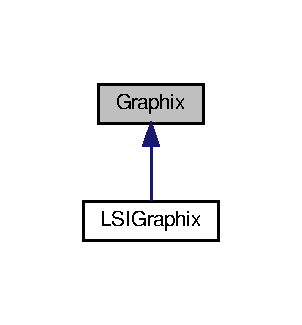
\includegraphics[width=145pt]{classGraphix__inherit__graph}
\end{center}
\end{figure}
\subsection*{Public Member Functions}
\begin{DoxyCompactItemize}
\item 
\hyperlink{classGraphix_a1d4cb173e0d22fee13a657489b7b55de}{Graphix} (std\+::mutex \&mtx)
\item 
void \hyperlink{classGraphix_a74af1cd957a0fc3b5e0ee1f951a994e1}{draw\+\_\+line} (\hyperlink{classLineSegment}{Line\+Segment} line, G\+Lfloat red=1, G\+Lfloat green=0, G\+Lfloat blue=0)
\item 
void \hyperlink{classGraphix_a9a1ebf0c6d508ce4686b9794c4dec871}{draw\+\_\+dashed\+\_\+line} (\hyperlink{classLineSegment}{Line\+Segment} line, G\+Lfloat red=0, G\+Lfloat green=0, G\+Lfloat blue=0)
\item 
void \hyperlink{classGraphix_af7b539b3ab40274dc2f89d060cba0c51}{loopie} ()
\item 
void \hyperlink{classGraphix_a3e24075d5ded3741a9c14a7978b721d8}{render} ()
\item 
void \hyperlink{classGraphix_a1ac1a5725a869ef074da6fe3cab29b0e}{clear} ()
\end{DoxyCompactItemize}
\subsection*{Public Attributes}
\begin{DoxyCompactItemize}
\item 
\mbox{\Hypertarget{classGraphix_ab2136667d30ca5f0017bceded579a803}\label{classGraphix_ab2136667d30ca5f0017bceded579a803}} 
std\+::mutex \& {\bfseries m\+\_\+mutex}
\item 
\mbox{\Hypertarget{classGraphix_a8189df95428d2fda74b1becb84ed07c2}\label{classGraphix_a8189df95428d2fda74b1becb84ed07c2}} 
G\+L\+F\+Wwindow $\ast$ {\bfseries window}
\end{DoxyCompactItemize}
\subsection*{Static Public Attributes}
\begin{DoxyCompactItemize}
\item 
\mbox{\Hypertarget{classGraphix_ab883fc83301f2a1a9d55b7ed8828bf66}\label{classGraphix_ab883fc83301f2a1a9d55b7ed8828bf66}} 
static bool {\bfseries pause\+\_\+flag} = true
\end{DoxyCompactItemize}


\subsection{Detailed Description}
Class for handling graphics using Open\+GL. 

\subsection{Constructor \& Destructor Documentation}
\mbox{\Hypertarget{classGraphix_a1d4cb173e0d22fee13a657489b7b55de}\label{classGraphix_a1d4cb173e0d22fee13a657489b7b55de}} 
\index{Graphix@{Graphix}!Graphix@{Graphix}}
\index{Graphix@{Graphix}!Graphix@{Graphix}}
\subsubsection{\texorpdfstring{Graphix()}{Graphix()}}
{\footnotesize\ttfamily Graphix\+::\+Graphix (\begin{DoxyParamCaption}\item[{std\+::mutex \&}]{mtx }\end{DoxyParamCaption})}

Constructor. Creates a window instance with default parameters. Ideally runs on a separate thread from the thread executing the core algorithm. Accept a reference to a mutex. Mutex is used to maintain synchronization between core algorithm execution and graphics handling functions. 
\begin{DoxyParams}{Parameters}
{\em m\+\_\+mutex} & Reference to a mutex object. \\
\hline
\end{DoxyParams}


\subsection{Member Function Documentation}
\mbox{\Hypertarget{classGraphix_a1ac1a5725a869ef074da6fe3cab29b0e}\label{classGraphix_a1ac1a5725a869ef074da6fe3cab29b0e}} 
\index{Graphix@{Graphix}!clear@{clear}}
\index{clear@{clear}!Graphix@{Graphix}}
\subsubsection{\texorpdfstring{clear()}{clear()}}
{\footnotesize\ttfamily void Graphix\+::clear (\begin{DoxyParamCaption}{ }\end{DoxyParamCaption})}

Utility function to clear the window. 
\begin{DoxyParams}{Parameters}
{\em line} & Object of \hyperlink{classLineSegment}{Line\+Segment} class. Holds description of line segment to be drawn. \\
\hline
\end{DoxyParams}
\mbox{\Hypertarget{classGraphix_a9a1ebf0c6d508ce4686b9794c4dec871}\label{classGraphix_a9a1ebf0c6d508ce4686b9794c4dec871}} 
\index{Graphix@{Graphix}!draw\+\_\+dashed\+\_\+line@{draw\+\_\+dashed\+\_\+line}}
\index{draw\+\_\+dashed\+\_\+line@{draw\+\_\+dashed\+\_\+line}!Graphix@{Graphix}}
\subsubsection{\texorpdfstring{draw\+\_\+dashed\+\_\+line()}{draw\_dashed\_line()}}
{\footnotesize\ttfamily void Graphix\+::draw\+\_\+dashed\+\_\+line (\begin{DoxyParamCaption}\item[{\hyperlink{classLineSegment}{Line\+Segment}}]{line,  }\item[{G\+Lfloat}]{red = {\ttfamily 0},  }\item[{G\+Lfloat}]{green = {\ttfamily 0},  }\item[{G\+Lfloat}]{blue = {\ttfamily 0} }\end{DoxyParamCaption})}

Utility function to draw a dashed/stippled line segment on the window. 
\begin{DoxyParams}{Parameters}
{\em line} & Object of \hyperlink{classLineSegment}{Line\+Segment} class. Holds description of line segment to be drawn. \\
\hline
\end{DoxyParams}
\mbox{\Hypertarget{classGraphix_a74af1cd957a0fc3b5e0ee1f951a994e1}\label{classGraphix_a74af1cd957a0fc3b5e0ee1f951a994e1}} 
\index{Graphix@{Graphix}!draw\+\_\+line@{draw\+\_\+line}}
\index{draw\+\_\+line@{draw\+\_\+line}!Graphix@{Graphix}}
\subsubsection{\texorpdfstring{draw\+\_\+line()}{draw\_line()}}
{\footnotesize\ttfamily void Graphix\+::draw\+\_\+line (\begin{DoxyParamCaption}\item[{\hyperlink{classLineSegment}{Line\+Segment}}]{line,  }\item[{G\+Lfloat}]{red = {\ttfamily 1},  }\item[{G\+Lfloat}]{green = {\ttfamily 0},  }\item[{G\+Lfloat}]{blue = {\ttfamily 0} }\end{DoxyParamCaption})}

Utility function to draw a line segment on the window. 
\begin{DoxyParams}{Parameters}
{\em line} & Object of \hyperlink{classLineSegment}{Line\+Segment} class. Holds description of line segment to be drawn. \\
\hline
\end{DoxyParams}
\mbox{\Hypertarget{classGraphix_af7b539b3ab40274dc2f89d060cba0c51}\label{classGraphix_af7b539b3ab40274dc2f89d060cba0c51}} 
\index{Graphix@{Graphix}!loopie@{loopie}}
\index{loopie@{loopie}!Graphix@{Graphix}}
\subsubsection{\texorpdfstring{loopie()}{loopie()}}
{\footnotesize\ttfamily void Graphix\+::loopie (\begin{DoxyParamCaption}{ }\end{DoxyParamCaption})}

Runs an infinite loop that listens to various events. \mbox{\Hypertarget{classGraphix_a3e24075d5ded3741a9c14a7978b721d8}\label{classGraphix_a3e24075d5ded3741a9c14a7978b721d8}} 
\index{Graphix@{Graphix}!render@{render}}
\index{render@{render}!Graphix@{Graphix}}
\subsubsection{\texorpdfstring{render()}{render()}}
{\footnotesize\ttfamily void Graphix\+::render (\begin{DoxyParamCaption}{ }\end{DoxyParamCaption})}

Renders whatever is on the buffer to the window. 

The documentation for this class was generated from the following files\+:\begin{DoxyCompactItemize}
\item 
src/graphix.\+h\item 
src/graphix.\+cpp\end{DoxyCompactItemize}

\hypertarget{classLineSegment}{}\section{Line\+Segment Class Reference}
\label{classLineSegment}\index{Line\+Segment@{Line\+Segment}}


Class for line segments.  




{\ttfamily \#include $<$primitives.\+h$>$}

\subsection*{Public Member Functions}
\begin{DoxyCompactItemize}
\item 
\hyperlink{classLineSegment_a691e185edf3aa7e2dc12307f9ef4be6b}{Line\+Segment} (\hyperlink{classPoint}{Point} p1, \hyperlink{classPoint}{Point} p2)
\begin{DoxyCompactList}\small\item\em Constructor, specifying two endpoints of the segment. \end{DoxyCompactList}\item 
bool \hyperlink{classLineSegment_a8dc46fa1dd259befff8cea92232e2a29}{contains\+\_\+point} (\hyperlink{classPoint}{Point} pt) const
\item 
\hyperlink{classPoint}{Point} \hyperlink{classLineSegment_a3bdc73ce4696a76b7c7dd143556c95b6}{intersects\+\_\+at} (\hyperlink{classLineSegment}{Line\+Segment} ls)
\item 
\hyperlink{classPoint}{Point} \hyperlink{classLineSegment_a51a9d2fcca6b3ff03cb51fd4d8fae4ba}{horizontal\+\_\+projection} (\hyperlink{classPoint}{Point} pt) const
\item 
bool \hyperlink{classLineSegment_ae73906b7230adbccf243c4b8dc6482b3}{operator==} (const \hyperlink{classLineSegment}{Line\+Segment} \&l2)
\item 
\hyperlink{classPoint}{Point} \hyperlink{classLineSegment_abe9136323cfe46be663907cbc1e3da2d}{start\+\_\+pt} () const
\item 
\hyperlink{classPoint}{Point} \hyperlink{classLineSegment_aa6c90340de500bb72bdde2114f838d57}{end\+\_\+pt} () const
\item 
bool \hyperlink{classLineSegment_a3364f7089cf7b650efe389475ddd0f12}{is\+\_\+nan} ()
\end{DoxyCompactItemize}
\subsection*{Friends}
\begin{DoxyCompactItemize}
\item 
\mbox{\Hypertarget{classLineSegment_aa6fe02d7d9f8ce3a0da5f6008b607850}\label{classLineSegment_aa6fe02d7d9f8ce3a0da5f6008b607850}} 
std\+::ostream \& {\bfseries operator$<$$<$} (std\+::ostream \&os, const \hyperlink{classLineSegment}{Line\+Segment} \&l)
\end{DoxyCompactItemize}


\subsection{Detailed Description}
Class for line segments. 

There is an inherent ordering between the two end points. So, initialising order in constructor does not affect the behaviour of the object 

\subsection{Constructor \& Destructor Documentation}
\mbox{\Hypertarget{classLineSegment_a691e185edf3aa7e2dc12307f9ef4be6b}\label{classLineSegment_a691e185edf3aa7e2dc12307f9ef4be6b}} 
\index{Line\+Segment@{Line\+Segment}!Line\+Segment@{Line\+Segment}}
\index{Line\+Segment@{Line\+Segment}!Line\+Segment@{Line\+Segment}}
\subsubsection{\texorpdfstring{Line\+Segment()}{LineSegment()}}
{\footnotesize\ttfamily Line\+Segment\+::\+Line\+Segment (\begin{DoxyParamCaption}\item[{\hyperlink{classPoint}{Point}}]{p1,  }\item[{\hyperlink{classPoint}{Point}}]{p2 }\end{DoxyParamCaption})}



Constructor, specifying two endpoints of the segment. 


\begin{DoxyParams}{Parameters}
{\em p1} & One endpoint of the line segment \\
\hline
{\em p2} & The other endpoint of the line segment \\
\hline
\end{DoxyParams}


\subsection{Member Function Documentation}
\mbox{\Hypertarget{classLineSegment_a8dc46fa1dd259befff8cea92232e2a29}\label{classLineSegment_a8dc46fa1dd259befff8cea92232e2a29}} 
\index{Line\+Segment@{Line\+Segment}!contains\+\_\+point@{contains\+\_\+point}}
\index{contains\+\_\+point@{contains\+\_\+point}!Line\+Segment@{Line\+Segment}}
\subsubsection{\texorpdfstring{contains\+\_\+point()}{contains\_point()}}
{\footnotesize\ttfamily bool Line\+Segment\+::contains\+\_\+point (\begin{DoxyParamCaption}\item[{\hyperlink{classPoint}{Point}}]{pt }\end{DoxyParamCaption}) const}

This function checks if a point lies on the given line segment. It returns true even if the point is onr of the endpoints of the line segment 
\begin{DoxyParams}{Parameters}
{\em pt} & \hyperlink{classPoint}{Point} to check \\
\hline
\end{DoxyParams}
\begin{DoxyReturn}{Returns}
true if point lies on line 
\end{DoxyReturn}
\mbox{\Hypertarget{classLineSegment_aa6c90340de500bb72bdde2114f838d57}\label{classLineSegment_aa6c90340de500bb72bdde2114f838d57}} 
\index{Line\+Segment@{Line\+Segment}!end\+\_\+pt@{end\+\_\+pt}}
\index{end\+\_\+pt@{end\+\_\+pt}!Line\+Segment@{Line\+Segment}}
\subsubsection{\texorpdfstring{end\+\_\+pt()}{end\_pt()}}
{\footnotesize\ttfamily \hyperlink{classPoint}{Point} Line\+Segment\+::end\+\_\+pt (\begin{DoxyParamCaption}{ }\end{DoxyParamCaption}) const}

Returns end point of the line segment Initialisation order does not matter \begin{DoxyReturn}{Returns}

\end{DoxyReturn}
\mbox{\Hypertarget{classLineSegment_a51a9d2fcca6b3ff03cb51fd4d8fae4ba}\label{classLineSegment_a51a9d2fcca6b3ff03cb51fd4d8fae4ba}} 
\index{Line\+Segment@{Line\+Segment}!horizontal\+\_\+projection@{horizontal\+\_\+projection}}
\index{horizontal\+\_\+projection@{horizontal\+\_\+projection}!Line\+Segment@{Line\+Segment}}
\subsubsection{\texorpdfstring{horizontal\+\_\+projection()}{horizontal\_projection()}}
{\footnotesize\ttfamily \hyperlink{classPoint}{Point} Line\+Segment\+::horizontal\+\_\+projection (\begin{DoxyParamCaption}\item[{\hyperlink{classPoint}{Point}}]{pt }\end{DoxyParamCaption}) const}

Returns a point that is a horizontal projection of the parameter point on the line segment. N\+A\+N\+\_\+\+P\+O\+I\+NT returned if no point found 
\begin{DoxyParams}{Parameters}
{\em pt} & \hyperlink{classPoint}{Point} whose horizontal projection we want to find \\
\hline
\end{DoxyParams}
\begin{DoxyReturn}{Returns}
\hyperlink{classPoint}{Point} which is horizontal projection of the 

N\+A\+N\+\_\+\+P\+O\+I\+NT if no projection 
\end{DoxyReturn}
\mbox{\Hypertarget{classLineSegment_a3bdc73ce4696a76b7c7dd143556c95b6}\label{classLineSegment_a3bdc73ce4696a76b7c7dd143556c95b6}} 
\index{Line\+Segment@{Line\+Segment}!intersects\+\_\+at@{intersects\+\_\+at}}
\index{intersects\+\_\+at@{intersects\+\_\+at}!Line\+Segment@{Line\+Segment}}
\subsubsection{\texorpdfstring{intersects\+\_\+at()}{intersects\_at()}}
{\footnotesize\ttfamily \hyperlink{classPoint}{Point} Line\+Segment\+::intersects\+\_\+at (\begin{DoxyParamCaption}\item[{\hyperlink{classLineSegment}{Line\+Segment}}]{ls }\end{DoxyParamCaption})}


\begin{DoxyParams}{Parameters}
{\em ls} & The line segment to check with \\
\hline
\end{DoxyParams}
\begin{DoxyReturn}{Returns}
\hyperlink{classPoint}{Point} where the two line segments intersect 

N\+A\+N\+\_\+\+P\+O\+I\+NT if the segments dont intersect 
\end{DoxyReturn}
\mbox{\Hypertarget{classLineSegment_a3364f7089cf7b650efe389475ddd0f12}\label{classLineSegment_a3364f7089cf7b650efe389475ddd0f12}} 
\index{Line\+Segment@{Line\+Segment}!is\+\_\+nan@{is\+\_\+nan}}
\index{is\+\_\+nan@{is\+\_\+nan}!Line\+Segment@{Line\+Segment}}
\subsubsection{\texorpdfstring{is\+\_\+nan()}{is\_nan()}}
{\footnotesize\ttfamily bool Line\+Segment\+::is\+\_\+nan (\begin{DoxyParamCaption}{ }\end{DoxyParamCaption})}

\begin{DoxyReturn}{Returns}
true if line segment is N\+A\+N\+\_\+\+L\+I\+NE 
\end{DoxyReturn}
\mbox{\Hypertarget{classLineSegment_ae73906b7230adbccf243c4b8dc6482b3}\label{classLineSegment_ae73906b7230adbccf243c4b8dc6482b3}} 
\index{Line\+Segment@{Line\+Segment}!operator==@{operator==}}
\index{operator==@{operator==}!Line\+Segment@{Line\+Segment}}
\subsubsection{\texorpdfstring{operator==()}{operator==()}}
{\footnotesize\ttfamily bool Line\+Segment\+::operator== (\begin{DoxyParamCaption}\item[{const \hyperlink{classLineSegment}{Line\+Segment} \&}]{l2 }\end{DoxyParamCaption})}

Two lines are equal if they have the same endpoints 
\begin{DoxyParams}{Parameters}
{\em l2} & \\
\hline
\end{DoxyParams}
\begin{DoxyReturn}{Returns}
true if the two line segments are the same 
\end{DoxyReturn}
\mbox{\Hypertarget{classLineSegment_abe9136323cfe46be663907cbc1e3da2d}\label{classLineSegment_abe9136323cfe46be663907cbc1e3da2d}} 
\index{Line\+Segment@{Line\+Segment}!start\+\_\+pt@{start\+\_\+pt}}
\index{start\+\_\+pt@{start\+\_\+pt}!Line\+Segment@{Line\+Segment}}
\subsubsection{\texorpdfstring{start\+\_\+pt()}{start\_pt()}}
{\footnotesize\ttfamily \hyperlink{classPoint}{Point} Line\+Segment\+::start\+\_\+pt (\begin{DoxyParamCaption}{ }\end{DoxyParamCaption}) const}

Returns start point of the line segment Initialisation order does not matter \begin{DoxyReturn}{Returns}

\end{DoxyReturn}


The documentation for this class was generated from the following files\+:\begin{DoxyCompactItemize}
\item 
src/primitives.\+h\item 
src/primitives.\+cpp\end{DoxyCompactItemize}

\hypertarget{classLineSegmentIntersector}{}\section{Line\+Segment\+Intersector Class Reference}
\label{classLineSegmentIntersector}\index{Line\+Segment\+Intersector@{Line\+Segment\+Intersector}}


Collaboration diagram for Line\+Segment\+Intersector\+:
\nopagebreak
\begin{figure}[H]
\begin{center}
\leavevmode
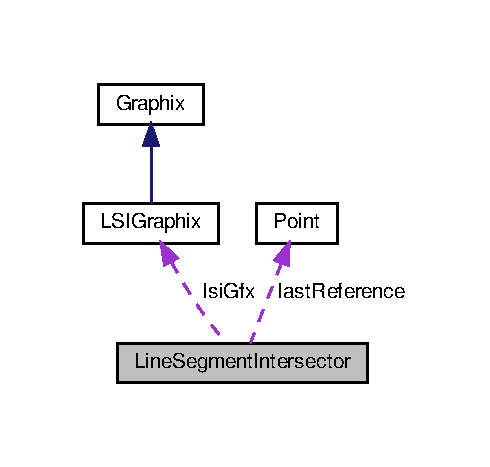
\includegraphics[width=235pt]{classLineSegmentIntersector__coll__graph}
\end{center}
\end{figure}
\subsection*{Public Member Functions}
\begin{DoxyCompactItemize}
\item 
\hyperlink{classLineSegmentIntersector_abfe17083938ad4ee705fbe7d0051f209}{Line\+Segment\+Intersector} (std\+::vector$<$ \hyperlink{classLineSegment}{Line\+Segment} $>$ \&, \hyperlink{classLSIGraphix}{L\+S\+I\+Graphix} \&)
\item 
L\+S\+I\+Result \hyperlink{classLineSegmentIntersector_a261dcce43777e1954e81589ca89529ee}{compute\+Intersections} ()
\end{DoxyCompactItemize}
\subsection*{Public Attributes}
\begin{DoxyCompactItemize}
\item 
\mbox{\Hypertarget{classLineSegmentIntersector_a82113ff9c3ccbf2c276c67a45401430a}\label{classLineSegmentIntersector_a82113ff9c3ccbf2c276c67a45401430a}} 
\hyperlink{classLSIGraphix}{L\+S\+I\+Graphix} \& {\bfseries lsi\+Gfx}
\end{DoxyCompactItemize}
\subsection*{Static Public Attributes}
\begin{DoxyCompactItemize}
\item 
\mbox{\Hypertarget{classLineSegmentIntersector_a170c7914f53e24387e8e46cedf3a1290}\label{classLineSegmentIntersector_a170c7914f53e24387e8e46cedf3a1290}} 
static \hyperlink{classPoint}{Point} {\bfseries last\+Reference} = N\+A\+N\+\_\+\+P\+O\+I\+NT
\end{DoxyCompactItemize}
\subsection*{Friends}
\begin{DoxyCompactItemize}
\item 
\mbox{\Hypertarget{classLineSegmentIntersector_ac30b368f45ebad37982a7529f590c24d}\label{classLineSegmentIntersector_ac30b368f45ebad37982a7529f590c24d}} 
std\+::ostream \& {\bfseries operator$<$$<$} (std\+::ostream \&os, const L\+S\+I\+Segment \&lsi\+Segment)
\item 
\mbox{\Hypertarget{classLineSegmentIntersector_aa1641902c18c0376d0303883d4e759e5}\label{classLineSegmentIntersector_aa1641902c18c0376d0303883d4e759e5}} 
void {\bfseries swap} (L\+S\+I\+Point \&, L\+S\+I\+Point \&)
\end{DoxyCompactItemize}


\subsection{Constructor \& Destructor Documentation}
\mbox{\Hypertarget{classLineSegmentIntersector_abfe17083938ad4ee705fbe7d0051f209}\label{classLineSegmentIntersector_abfe17083938ad4ee705fbe7d0051f209}} 
\index{Line\+Segment\+Intersector@{Line\+Segment\+Intersector}!Line\+Segment\+Intersector@{Line\+Segment\+Intersector}}
\index{Line\+Segment\+Intersector@{Line\+Segment\+Intersector}!Line\+Segment\+Intersector@{Line\+Segment\+Intersector}}
\subsubsection{\texorpdfstring{Line\+Segment\+Intersector()}{LineSegmentIntersector()}}
{\footnotesize\ttfamily Line\+Segment\+Intersector\+::\+Line\+Segment\+Intersector (\begin{DoxyParamCaption}\item[{std\+::vector$<$ \hyperlink{classLineSegment}{Line\+Segment} $>$ \&}]{i,  }\item[{\hyperlink{classLSIGraphix}{L\+S\+I\+Graphix} \&}]{l }\end{DoxyParamCaption})}

Pass the set of points and L\+SI Visualizer Object 

\subsection{Member Function Documentation}
\mbox{\Hypertarget{classLineSegmentIntersector_a261dcce43777e1954e81589ca89529ee}\label{classLineSegmentIntersector_a261dcce43777e1954e81589ca89529ee}} 
\index{Line\+Segment\+Intersector@{Line\+Segment\+Intersector}!compute\+Intersections@{compute\+Intersections}}
\index{compute\+Intersections@{compute\+Intersections}!Line\+Segment\+Intersector@{Line\+Segment\+Intersector}}
\subsubsection{\texorpdfstring{compute\+Intersections()}{computeIntersections()}}
{\footnotesize\ttfamily L\+S\+I\+Result Line\+Segment\+Intersector\+::compute\+Intersections (\begin{DoxyParamCaption}{ }\end{DoxyParamCaption})}

This computes the intersection point and visualizes it. \begin{DoxyReturn}{Returns}
intersection points and all points that pass though it 
\end{DoxyReturn}


The documentation for this class was generated from the following files\+:\begin{DoxyCompactItemize}
\item 
src/Line\+Segment\+Intersector.\+h\item 
src/Line\+Segment\+Intersector.\+cpp\end{DoxyCompactItemize}

\hypertarget{classLSIGraphix}{}\section{L\+S\+I\+Graphix Class Reference}
\label{classLSIGraphix}\index{L\+S\+I\+Graphix@{L\+S\+I\+Graphix}}


Class for especially handling events for Bentley-\/\+Ottoman Algorithm. Inherits \hyperlink{classGraphix}{Graphix} class.  




{\ttfamily \#include $<$L\+S\+I\+Graphix.\+h$>$}



Inheritance diagram for L\+S\+I\+Graphix\+:
% FIG 0


Collaboration diagram for L\+S\+I\+Graphix\+:
% FIG 1
\subsection*{Public Member Functions}
\begin{DoxyCompactItemize}
\item 
\hyperlink{classLSIGraphix_a36adc59a5f2f87571cb230de95e0c0bc}{L\+S\+I\+Graphix} (std\+::mutex \&mtx)
\item 
void \hyperlink{classLSIGraphix_aa95fa264bddca976f974f6eae9173444}{init\+\_\+lines} (std\+::vector$<$ \hyperlink{classLineSegment}{Line\+Segment} $>$ lines)
\item 
void \hyperlink{classLSIGraphix_a136dca7736d6a885ef9b40824808c447}{update\+\_\+event} (\hyperlink{classPoint}{Point})
\end{DoxyCompactItemize}
\subsection*{Additional Inherited Members}


\subsection{Detailed Description}
Class for especially handling events for Bentley-\/\+Ottoman Algorithm. Inherits \hyperlink{classGraphix}{Graphix} class. 

\subsection{Constructor \& Destructor Documentation}
\mbox{\Hypertarget{classLSIGraphix_a36adc59a5f2f87571cb230de95e0c0bc}\label{classLSIGraphix_a36adc59a5f2f87571cb230de95e0c0bc}} 
\index{L\+S\+I\+Graphix@{L\+S\+I\+Graphix}!L\+S\+I\+Graphix@{L\+S\+I\+Graphix}}
\index{L\+S\+I\+Graphix@{L\+S\+I\+Graphix}!L\+S\+I\+Graphix@{L\+S\+I\+Graphix}}
\subsubsection{\texorpdfstring{L\+S\+I\+Graphix()}{LSIGraphix()}}
{\footnotesize\ttfamily L\+S\+I\+Graphix\+::\+L\+S\+I\+Graphix (\begin{DoxyParamCaption}\item[{std\+::mutex \&}]{mtx }\end{DoxyParamCaption})}

Constructor. Calls super class \hyperlink{classGraphix}{Graphix} constructor by passing mutex object and initiates a sweep line. 

\subsection{Member Function Documentation}
\mbox{\Hypertarget{classLSIGraphix_aa95fa264bddca976f974f6eae9173444}\label{classLSIGraphix_aa95fa264bddca976f974f6eae9173444}} 
\index{L\+S\+I\+Graphix@{L\+S\+I\+Graphix}!init\+\_\+lines@{init\+\_\+lines}}
\index{init\+\_\+lines@{init\+\_\+lines}!L\+S\+I\+Graphix@{L\+S\+I\+Graphix}}
\subsubsection{\texorpdfstring{init\+\_\+lines()}{init\_lines()}}
{\footnotesize\ttfamily void L\+S\+I\+Graphix\+::init\+\_\+lines (\begin{DoxyParamCaption}\item[{std\+::vector$<$ \hyperlink{classLineSegment}{Line\+Segment} $>$}]{lines }\end{DoxyParamCaption})}

Updates list of input lines to be drawn. 
\begin{DoxyParams}{Parameters}
{\em lines} & updated set of lines \\
\hline
\end{DoxyParams}
\mbox{\Hypertarget{classLSIGraphix_a136dca7736d6a885ef9b40824808c447}\label{classLSIGraphix_a136dca7736d6a885ef9b40824808c447}} 
\index{L\+S\+I\+Graphix@{L\+S\+I\+Graphix}!update\+\_\+event@{update\+\_\+event}}
\index{update\+\_\+event@{update\+\_\+event}!L\+S\+I\+Graphix@{L\+S\+I\+Graphix}}
\subsubsection{\texorpdfstring{update\+\_\+event()}{update\_event()}}
{\footnotesize\ttfamily void L\+S\+I\+Graphix\+::update\+\_\+event (\begin{DoxyParamCaption}\item[{\hyperlink{classPoint}{Point}}]{pt }\end{DoxyParamCaption})}

Updates event point and sweep line in the window buffer. 
\begin{DoxyParams}{Parameters}
{\em \hyperlink{classPoint}{Point}} & New event point. \\
\hline
\end{DoxyParams}


The documentation for this class was generated from the following files\+:\begin{DoxyCompactItemize}
\item 
src/L\+S\+I\+Graphix.\+h\item 
src/L\+S\+I\+Graphix.\+cpp\end{DoxyCompactItemize}

\hypertarget{classLineSegmentIntersector_1_1LSIPoint}{}\section{Line\+Segment\+Intersector\+:\+:L\+S\+I\+Point Class Reference}
\label{classLineSegmentIntersector_1_1LSIPoint}\index{Line\+Segment\+Intersector\+::\+L\+S\+I\+Point@{Line\+Segment\+Intersector\+::\+L\+S\+I\+Point}}


Inheritance diagram for Line\+Segment\+Intersector\+:\+:L\+S\+I\+Point\+:
\nopagebreak
\begin{figure}[H]
\begin{center}
\leavevmode
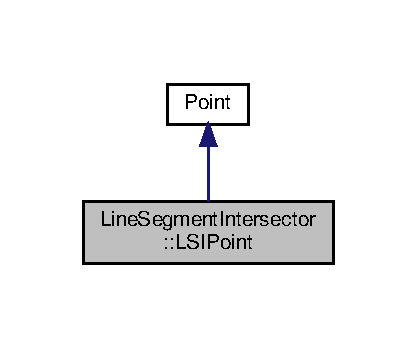
\includegraphics[width=200pt]{classLineSegmentIntersector_1_1LSIPoint__inherit__graph}
\end{center}
\end{figure}


Collaboration diagram for Line\+Segment\+Intersector\+:\+:L\+S\+I\+Point\+:
\nopagebreak
\begin{figure}[H]
\begin{center}
\leavevmode
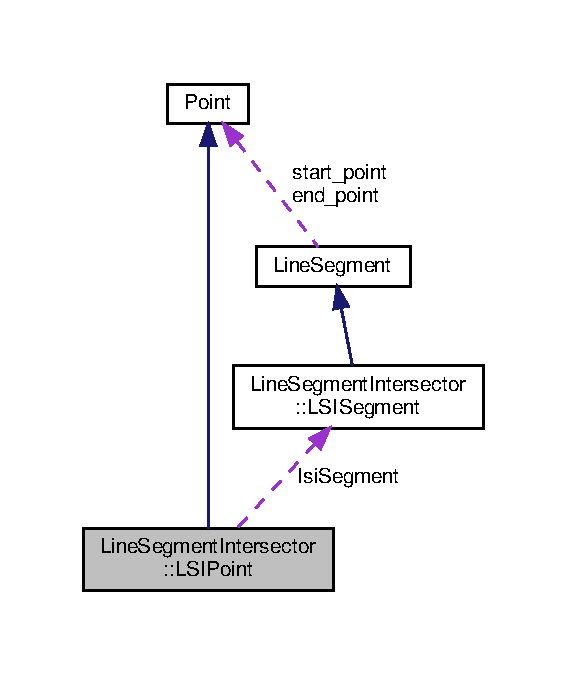
\includegraphics[width=272pt]{classLineSegmentIntersector_1_1LSIPoint__coll__graph}
\end{center}
\end{figure}
\subsection*{Public Member Functions}
\begin{DoxyCompactItemize}
\item 
\mbox{\Hypertarget{classLineSegmentIntersector_1_1LSIPoint_a1b3ac13032c42bad86516cbcf953db66}\label{classLineSegmentIntersector_1_1LSIPoint_a1b3ac13032c42bad86516cbcf953db66}} 
bool {\bfseries operator$<$} (\hyperlink{classLineSegmentIntersector_1_1LSIPoint}{L\+S\+I\+Point})
\item 
\mbox{\Hypertarget{classLineSegmentIntersector_1_1LSIPoint_ac547954aaa117fd416bb84a4a7447e56}\label{classLineSegmentIntersector_1_1LSIPoint_ac547954aaa117fd416bb84a4a7447e56}} 
\hyperlink{classLineSegmentIntersector_1_1LSIPoint}{L\+S\+I\+Point} \& {\bfseries operator=} (\hyperlink{classLineSegmentIntersector_1_1LSIPoint}{L\+S\+I\+Point} \&)
\item 
\mbox{\Hypertarget{classLineSegmentIntersector_1_1LSIPoint_a00b901f7dd62d86e3523c6592e9c1514}\label{classLineSegmentIntersector_1_1LSIPoint_a00b901f7dd62d86e3523c6592e9c1514}} 
{\bfseries L\+S\+I\+Point} (\hyperlink{classPoint}{Point}, \hyperlink{classLineSegmentIntersector_1_1LSISegment}{L\+S\+I\+Segment}, Event\+Type)
\end{DoxyCompactItemize}
\subsection*{Public Attributes}
\begin{DoxyCompactItemize}
\item 
\mbox{\Hypertarget{classLineSegmentIntersector_1_1LSIPoint_ab84e13cb9e39eeca6d8af71d4b09582d}\label{classLineSegmentIntersector_1_1LSIPoint_ab84e13cb9e39eeca6d8af71d4b09582d}} 
\hyperlink{classLineSegmentIntersector_1_1LSISegment}{L\+S\+I\+Segment} {\bfseries lsi\+Segment}
\item 
\mbox{\Hypertarget{classLineSegmentIntersector_1_1LSIPoint_a01054b1139f1e58e5af7b45213dd3c57}\label{classLineSegmentIntersector_1_1LSIPoint_a01054b1139f1e58e5af7b45213dd3c57}} 
Event\+Type {\bfseries et}
\end{DoxyCompactItemize}


The documentation for this class was generated from the following files\+:\begin{DoxyCompactItemize}
\item 
src/Line\+Segment\+Intersector.\+h\item 
src/Line\+Segment\+Intersector.\+cpp\end{DoxyCompactItemize}

\hypertarget{classLineSegmentIntersector_1_1LSISegment}{}\section{Line\+Segment\+Intersector\+:\+:L\+S\+I\+Segment Class Reference}
\label{classLineSegmentIntersector_1_1LSISegment}\index{Line\+Segment\+Intersector\+::\+L\+S\+I\+Segment@{Line\+Segment\+Intersector\+::\+L\+S\+I\+Segment}}


Inheritance diagram for Line\+Segment\+Intersector\+:\+:L\+S\+I\+Segment\+:
% FIG 0


Collaboration diagram for Line\+Segment\+Intersector\+:\+:L\+S\+I\+Segment\+:
% FIG 1
\subsection*{Public Member Functions}
\begin{DoxyCompactItemize}
\item 
\mbox{\Hypertarget{classLineSegmentIntersector_1_1LSISegment_a9849ef126f6018d8ebf789e7c216801d}\label{classLineSegmentIntersector_1_1LSISegment_a9849ef126f6018d8ebf789e7c216801d}} 
bool {\bfseries operator$<$} (const \hyperlink{classLineSegmentIntersector_1_1LSISegment}{L\+S\+I\+Segment} \&) const
\item 
\mbox{\Hypertarget{classLineSegmentIntersector_1_1LSISegment_a46caed8fba72da47df4586d06197b33a}\label{classLineSegmentIntersector_1_1LSISegment_a46caed8fba72da47df4586d06197b33a}} 
bool {\bfseries operator$>$} (const \hyperlink{classLineSegmentIntersector_1_1LSISegment}{L\+S\+I\+Segment} \&) const
\item 
\mbox{\Hypertarget{classLineSegmentIntersector_1_1LSISegment_a3771a4e4e29f239f5614909a86df824b}\label{classLineSegmentIntersector_1_1LSISegment_a3771a4e4e29f239f5614909a86df824b}} 
bool {\bfseries operator!=} (const \hyperlink{classLineSegmentIntersector_1_1LSISegment}{L\+S\+I\+Segment} \&) const
\item 
\mbox{\Hypertarget{classLineSegmentIntersector_1_1LSISegment_a001a3f2f7335f4f979b8d7f680ffbe9e}\label{classLineSegmentIntersector_1_1LSISegment_a001a3f2f7335f4f979b8d7f680ffbe9e}} 
bool {\bfseries operator$<$=} (const \hyperlink{classLineSegmentIntersector_1_1LSISegment}{L\+S\+I\+Segment} \&) const
\item 
\mbox{\Hypertarget{classLineSegmentIntersector_1_1LSISegment_a4c6fd956e9c6b9c5cf6f27b9ffc89726}\label{classLineSegmentIntersector_1_1LSISegment_a4c6fd956e9c6b9c5cf6f27b9ffc89726}} 
{\bfseries L\+S\+I\+Segment} (\hyperlink{classLineSegment}{Line\+Segment})
\item 
\mbox{\Hypertarget{classLineSegmentIntersector_1_1LSISegment_a9797f919e76bb5de2ccff9adc651ed91}\label{classLineSegmentIntersector_1_1LSISegment_a9797f919e76bb5de2ccff9adc651ed91}} 
\hyperlink{classLineSegmentIntersector_1_1LSISegment}{L\+S\+I\+Segment} \& {\bfseries operator=} (\hyperlink{classLineSegmentIntersector_1_1LSISegment}{L\+S\+I\+Segment} \&)
\end{DoxyCompactItemize}
\subsection*{Additional Inherited Members}


The documentation for this class was generated from the following files\+:\begin{DoxyCompactItemize}
\item 
src/Line\+Segment\+Intersector.\+h\item 
src/Line\+Segment\+Intersector.\+cpp\end{DoxyCompactItemize}

\hypertarget{classPoint}{}\section{Point Class Reference}
\label{classPoint}\index{Point@{Point}}


Stores point with X \& Y coordinate.  




{\ttfamily \#include $<$primitives.\+h$>$}

\subsection*{Public Member Functions}
\begin{DoxyCompactItemize}
\item 
\hyperlink{classPoint_ad92f2337b839a94ce97dcdb439b4325a}{Point} ()
\item 
\hyperlink{classPoint_af7373698b9fafc53b0a5d06e511642e1}{Point} (coordinate x\+\_\+in, coordinate y\+\_\+in)
\item 
\hyperlink{classPoint}{Point} \& \hyperlink{classPoint_a2e142edc132377fdc6873f6549daab2d}{operator=} (const \hyperlink{classPoint}{Point} \&op)
\item 
bool \hyperlink{classPoint_ac7bc64b9a683d5fb35780c739779f2fc}{operator==} (const \hyperlink{classPoint}{Point} \&p2)
\item 
bool \hyperlink{classPoint_ade5f3908ec0e412aea8c3e12f5d0e26f}{operator!=} (const \hyperlink{classPoint}{Point} \&p2)
\item 
bool \hyperlink{classPoint_a2d285a505e84d64a96974d5247e8ae7a}{operator$<$} (const \hyperlink{classPoint}{Point} \&right) const
\item 
bool \hyperlink{classPoint_a2bc8aed929f6be2b543ba2f26b8a5f72}{is\+\_\+nan} ()
\end{DoxyCompactItemize}
\subsection*{Public Attributes}
\begin{DoxyCompactItemize}
\item 
coordinate \hyperlink{classPoint_a2e5bf2da8d7f35ef2ca707ae5ec1929b}{x}
\item 
coordinate \hyperlink{classPoint_a4390d37c7ed19ad07212fc84df2fe26e}{y}
\end{DoxyCompactItemize}
\subsection*{Friends}
\begin{DoxyCompactItemize}
\item 
\mbox{\Hypertarget{classPoint_a2c120859855730a5ff9d2eaee48471c5}\label{classPoint_a2c120859855730a5ff9d2eaee48471c5}} 
std\+::ostream \& {\bfseries operator$<$$<$} (std\+::ostream \&os, const \hyperlink{classPoint}{Point} \&pt)
\end{DoxyCompactItemize}


\subsection{Detailed Description}
Stores point with X \& Y coordinate. 

\subsection{Constructor \& Destructor Documentation}
\mbox{\Hypertarget{classPoint_ad92f2337b839a94ce97dcdb439b4325a}\label{classPoint_ad92f2337b839a94ce97dcdb439b4325a}} 
\index{Point@{Point}!Point@{Point}}
\index{Point@{Point}!Point@{Point}}
\subsubsection{\texorpdfstring{Point()}{Point()}\hspace{0.1cm}{\footnotesize\ttfamily [1/2]}}
{\footnotesize\ttfamily Point\+::\+Point (\begin{DoxyParamCaption}{ }\end{DoxyParamCaption})}

Constructor, makes a point with x \& y coordinates 0 \mbox{\Hypertarget{classPoint_af7373698b9fafc53b0a5d06e511642e1}\label{classPoint_af7373698b9fafc53b0a5d06e511642e1}} 
\index{Point@{Point}!Point@{Point}}
\index{Point@{Point}!Point@{Point}}
\subsubsection{\texorpdfstring{Point()}{Point()}\hspace{0.1cm}{\footnotesize\ttfamily [2/2]}}
{\footnotesize\ttfamily Point\+::\+Point (\begin{DoxyParamCaption}\item[{coordinate}]{x\+\_\+in,  }\item[{coordinate}]{y\+\_\+in }\end{DoxyParamCaption})}


\begin{DoxyParams}{Parameters}
{\em x\+\_\+in} & \+: X coordinate of point \\
\hline
{\em y\+\_\+in} & \+: Y coordinate of point \\
\hline
\end{DoxyParams}


\subsection{Member Function Documentation}
\mbox{\Hypertarget{classPoint_a2bc8aed929f6be2b543ba2f26b8a5f72}\label{classPoint_a2bc8aed929f6be2b543ba2f26b8a5f72}} 
\index{Point@{Point}!is\+\_\+nan@{is\+\_\+nan}}
\index{is\+\_\+nan@{is\+\_\+nan}!Point@{Point}}
\subsubsection{\texorpdfstring{is\+\_\+nan()}{is\_nan()}}
{\footnotesize\ttfamily bool Point\+::is\+\_\+nan (\begin{DoxyParamCaption}{ }\end{DoxyParamCaption})}

Checks if a point is a N\+A\+N\+\_\+\+P\+O\+I\+NT \begin{DoxyReturn}{Returns}
true if point is a N\+A\+N\+\_\+\+P\+O\+I\+NT 
\end{DoxyReturn}
\mbox{\Hypertarget{classPoint_ade5f3908ec0e412aea8c3e12f5d0e26f}\label{classPoint_ade5f3908ec0e412aea8c3e12f5d0e26f}} 
\index{Point@{Point}!operator"!=@{operator"!=}}
\index{operator"!=@{operator"!=}!Point@{Point}}
\subsubsection{\texorpdfstring{operator"!=()}{operator!=()}}
{\footnotesize\ttfamily bool Point\+::operator!= (\begin{DoxyParamCaption}\item[{const \hyperlink{classPoint}{Point} \&}]{p2 }\end{DoxyParamCaption})}

Overloaded != operator. Refer to = for point 
\begin{DoxyParams}{Parameters}
{\em p2} & -\/ \hyperlink{classPoint}{Point} to be compared with \\
\hline
\end{DoxyParams}
\begin{DoxyReturn}{Returns}
true if points have at least one different coordinate 
\end{DoxyReturn}
\mbox{\Hypertarget{classPoint_a2d285a505e84d64a96974d5247e8ae7a}\label{classPoint_a2d285a505e84d64a96974d5247e8ae7a}} 
\index{Point@{Point}!operator$<$@{operator$<$}}
\index{operator$<$@{operator$<$}!Point@{Point}}
\subsubsection{\texorpdfstring{operator$<$()}{operator<()}}
{\footnotesize\ttfamily bool Point\+::operator$<$ (\begin{DoxyParamCaption}\item[{const \hyperlink{classPoint}{Point} \&}]{right }\end{DoxyParamCaption}) const}

This operator does not have any semantic meaning A hard ordering of points has been done to ensure Points can be inserted into S\+TL containers 
\begin{DoxyParams}{Parameters}
{\em right} & \\
\hline
\end{DoxyParams}
\begin{DoxyReturn}{Returns}
bool 
\end{DoxyReturn}
\mbox{\Hypertarget{classPoint_a2e142edc132377fdc6873f6549daab2d}\label{classPoint_a2e142edc132377fdc6873f6549daab2d}} 
\index{Point@{Point}!operator=@{operator=}}
\index{operator=@{operator=}!Point@{Point}}
\subsubsection{\texorpdfstring{operator=()}{operator=()}}
{\footnotesize\ttfamily \hyperlink{classPoint}{Point} \& Point\+::operator= (\begin{DoxyParamCaption}\item[{const \hyperlink{classPoint}{Point} \&}]{op }\end{DoxyParamCaption})}

Standard overloading the = operator 
\begin{DoxyParams}{Parameters}
{\em op} & \\
\hline
\end{DoxyParams}
\begin{DoxyReturn}{Returns}
point with coordinates as that of input point 
\end{DoxyReturn}
\mbox{\Hypertarget{classPoint_ac7bc64b9a683d5fb35780c739779f2fc}\label{classPoint_ac7bc64b9a683d5fb35780c739779f2fc}} 
\index{Point@{Point}!operator==@{operator==}}
\index{operator==@{operator==}!Point@{Point}}
\subsubsection{\texorpdfstring{operator==()}{operator==()}}
{\footnotesize\ttfamily bool Point\+::operator== (\begin{DoxyParamCaption}\item[{const \hyperlink{classPoint}{Point} \&}]{p2 }\end{DoxyParamCaption})}

Two points are equal if they have same x \& y coordinates 
\begin{DoxyParams}{Parameters}
{\em p2} & \\
\hline
\end{DoxyParams}
\begin{DoxyReturn}{Returns}
true if the points are same 
\end{DoxyReturn}


\subsection{Member Data Documentation}
\mbox{\Hypertarget{classPoint_a2e5bf2da8d7f35ef2ca707ae5ec1929b}\label{classPoint_a2e5bf2da8d7f35ef2ca707ae5ec1929b}} 
\index{Point@{Point}!x@{x}}
\index{x@{x}!Point@{Point}}
\subsubsection{\texorpdfstring{x}{x}}
{\footnotesize\ttfamily coordinate Point\+::x}

the X coordinate of the point can be accessed publicly \mbox{\Hypertarget{classPoint_a4390d37c7ed19ad07212fc84df2fe26e}\label{classPoint_a4390d37c7ed19ad07212fc84df2fe26e}} 
\index{Point@{Point}!y@{y}}
\index{y@{y}!Point@{Point}}
\subsubsection{\texorpdfstring{y}{y}}
{\footnotesize\ttfamily coordinate Point\+::y}

the X coordinate of the point can be accessed publicly 

The documentation for this class was generated from the following files\+:\begin{DoxyCompactItemize}
\item 
src/primitives.\+h\item 
src/primitives.\+cpp\end{DoxyCompactItemize}

\hypertarget{classStatus}{}\section{Status$<$ T $>$ Class Template Reference}
\label{classStatus}\index{Status$<$ T $>$@{Status$<$ T $>$}}


{\ttfamily \#include $<$Status.\+h$>$}

\subsection*{Public Member Functions}
\begin{DoxyCompactItemize}
\item 
void \hyperlink{classStatus_aa019369b98450d3003f6359003fcb348}{inorder} ()
\item 
void \hyperlink{classStatus_a5fd5e49c03713d3b918010a15595d169}{insert} (T)
\item 
void \hyperlink{classStatus_afe333856c09425b4e0c7071ab4a700a5}{remove} (T)
\item 
T $\ast$ \hyperlink{classStatus_a0b6a56cd7787478d30814c372ce7aff3}{searchL} (T)
\item 
T $\ast$ \hyperlink{classStatus_a8db67cdc477f8f55b5c16678b2ec27f0}{searchR} (T)
\end{DoxyCompactItemize}


\subsection{Detailed Description}
\subsubsection*{template$<$class T$>$\newline
class Status$<$ T $>$}

\hyperlink{classStatus}{Status} is a balanced tree, that allows for neighbour search 
\begin{DoxyTemplParams}{Template Parameters}
{\em T} & \+: template class for which you want to build the status \\
\hline
\end{DoxyTemplParams}


\subsection{Member Function Documentation}
\mbox{\Hypertarget{classStatus_aa019369b98450d3003f6359003fcb348}\label{classStatus_aa019369b98450d3003f6359003fcb348}} 
\index{Status@{Status}!inorder@{inorder}}
\index{inorder@{inorder}!Status@{Status}}
\subsubsection{\texorpdfstring{inorder()}{inorder()}}
{\footnotesize\ttfamily template$<$class T $>$ \\
void \hyperlink{classStatus}{Status}$<$ T $>$\+::inorder (\begin{DoxyParamCaption}{ }\end{DoxyParamCaption})}

Prints inorder traversal Requires that operator$<$$<$ for ostream be overloaded for $<$ T $>$ class \mbox{\Hypertarget{classStatus_a5fd5e49c03713d3b918010a15595d169}\label{classStatus_a5fd5e49c03713d3b918010a15595d169}} 
\index{Status@{Status}!insert@{insert}}
\index{insert@{insert}!Status@{Status}}
\subsubsection{\texorpdfstring{insert()}{insert()}}
{\footnotesize\ttfamily template$<$class T$>$ \\
void \hyperlink{classStatus}{Status}$<$ T $>$\+::insert (\begin{DoxyParamCaption}\item[{T}]{key }\end{DoxyParamCaption})}

Insert an element into the tree 
\begin{DoxyParams}{Parameters}
{\em element} & to insert \\
\hline
\end{DoxyParams}
\mbox{\Hypertarget{classStatus_afe333856c09425b4e0c7071ab4a700a5}\label{classStatus_afe333856c09425b4e0c7071ab4a700a5}} 
\index{Status@{Status}!remove@{remove}}
\index{remove@{remove}!Status@{Status}}
\subsubsection{\texorpdfstring{remove()}{remove()}}
{\footnotesize\ttfamily template$<$class T$>$ \\
void \hyperlink{classStatus}{Status}$<$ T $>$\+::remove (\begin{DoxyParamCaption}\item[{T}]{key }\end{DoxyParamCaption})}

Removes element from tree Does nothing is element is not present \mbox{\Hypertarget{classStatus_a0b6a56cd7787478d30814c372ce7aff3}\label{classStatus_a0b6a56cd7787478d30814c372ce7aff3}} 
\index{Status@{Status}!searchL@{searchL}}
\index{searchL@{searchL}!Status@{Status}}
\subsubsection{\texorpdfstring{search\+L()}{searchL()}}
{\footnotesize\ttfamily template$<$class T$>$ \\
T $\ast$ \hyperlink{classStatus}{Status}$<$ T $>$\+::searchL (\begin{DoxyParamCaption}\item[{T}]{key }\end{DoxyParamCaption})}

Searches for element to the left of the param Returns null if no neighbour exists If param doesnt exist, we search for the smallest element greater than it 
\begin{DoxyParams}{Parameters}
{\em } & Element who\textquotesingle{}s left neighbour we want to search for\\
\hline
\end{DoxyParams}
Search the tree for left sibling of node with value key. \mbox{\Hypertarget{classStatus_a8db67cdc477f8f55b5c16678b2ec27f0}\label{classStatus_a8db67cdc477f8f55b5c16678b2ec27f0}} 
\index{Status@{Status}!searchR@{searchR}}
\index{searchR@{searchR}!Status@{Status}}
\subsubsection{\texorpdfstring{search\+R()}{searchR()}}
{\footnotesize\ttfamily template$<$class T$>$ \\
T $\ast$ \hyperlink{classStatus}{Status}$<$ T $>$\+::searchR (\begin{DoxyParamCaption}\item[{T}]{key }\end{DoxyParamCaption})}

Searches for element to the right of the param Returns null if no neighbour exists If param doesnt exist, we search for the smallest element greater than it 
\begin{DoxyParams}{Parameters}
{\em } & Element who\textquotesingle{}s right neighbour we want to search for\\
\hline
\end{DoxyParams}
Search the tree for right sibling of node with value key. 

The documentation for this class was generated from the following files\+:\begin{DoxyCompactItemize}
\item 
src/Status.\+h\item 
src/Status.\+cpp\end{DoxyCompactItemize}

\chapter{Example Documentation}
\hypertarget{Point-example}{}\section{Point}
p(3,5)\+: p is point with coordinates (3,5)


\begin{DoxyCodeInclude}
\end{DoxyCodeInclude}
 
%--- End generated contents ---

% Index
\backmatter
\newpage
\phantomsection
\clearemptydoublepage
\addcontentsline{toc}{chapter}{Index}
\printindex

\end{document}
